\title{Inferencing From Bayesian Networks\\Lab 5}
\author{
Aditya Gupta \\
\and
Milan Chaudhary
}
\date{\today}

\documentclass[12pt]{article}

\usepackage{tikz}
\usetikzlibrary{datavisualization}

\begin{document}
\maketitle

\section{Introduction}

\section{Variable Elimination}

\section{Rejection Sampling}
In this section of program, it will  n
\subsection{Convergence of the probabilities as function of\\ number of samples generated}
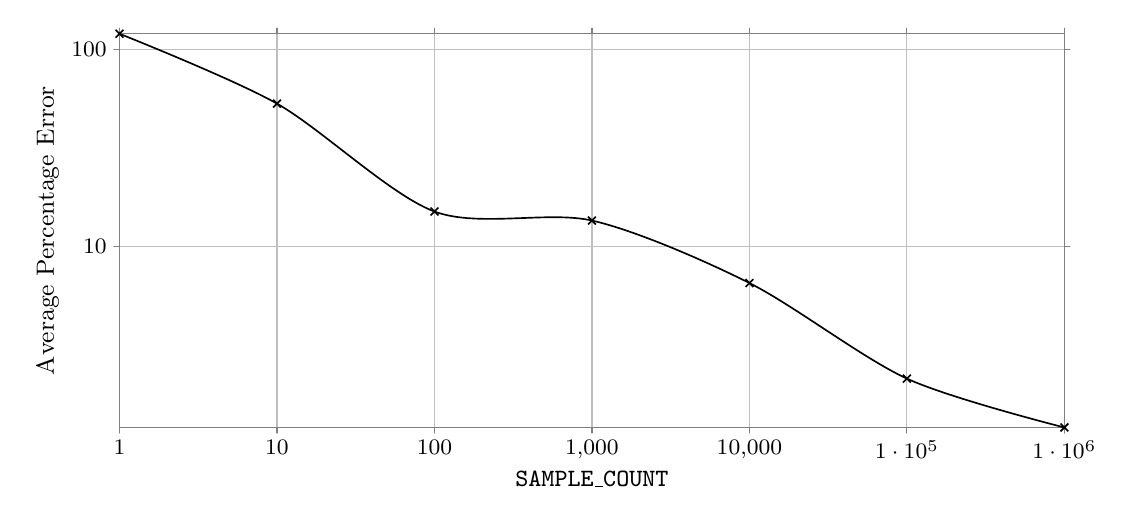
\begin{tikzpicture}
    \datavisualization [scientific axes,
    						 x axis={logarithmic,length=12cm,label=\texttt{SAMPLE\_COUNT},grid},
     						 y axis={logarithmic,length=5cm,label=Average Percentage Error,grid},
    						 visualize as smooth line=my data,
    						 my data={style={mark=x}}]
    data {
        x, y
        1, 120
        10, 53
        100, 15
        1000, 13.5
        10000, 6.5
        100000, 2.125
        1000000, 1.2
    };
\end{tikzpicture}

\end{document}
  
